%%%%%%%%%%%%%%%%%%%%%%%%%%%%%%%%%%%%%%%%%
%
% (c) 2020 by Jennifer Laaser
%
% This work is licensed under the Creative Commons Attribution-NonCommercial-ShareAlike 4.0 International License. To view a copy of this license, visit http://creativecommons.org/licenses/by-nc-sa/4.0/ or send a letter to Creative Commons, PO Box 1866, Mountain View, CA 94042, USA.
%
% The current source for these materials is accessible on Github: https://github.com/jlaaser/pogil-polymers
%
%%%%%%%%%%%%%%%%%%%%%%%%%%%%%%%%%%%%%%%%%

\renewcommand{\figpath}{content/intro/molecules-to-polymers/figs}
\renewcommand{\labelbase}{molecules-to-polymers}

\begin{activity}{From Molecules to Polymers}

\begin{instructornotes}

	This activity introduces students to the definition of the term \emph{polymer}, and key differences between small molecules and polymers.
	
	After completing this activity, students will be able to:
			\begin{enumerate}
				\item Define the term ``polymer''
				\item Write and interpret abbreviated skeletal structures for polymer chains
				\item Explain how the size of polymer molecules translates into changes in physical properties
			\end{enumerate}
			
	\subsection*{Activity summary:}
	\begin{itemize}
		\item \textbf{Activity type:} Learning Cycle
		\item \textbf{Content goals:} Introduction to polymers
		\item \textbf{Process goals:} %https://pogil.org/uploads/attachments/cj54b5yts006cklx4hh758htf-process-skills-official-pogil-list-2015-original.pdf
			written communication, critical thinking, information processing
		\item \textbf{Duration:} approx. 35 min including class discussion
	
		\item \textbf{Instructor preparation required:} none beyond knowledge of relevant content
		\item \textbf{Related textbook chapters:}
			\begin{itemize}
				\item \emph{Polymer Chemistry} (Hiemenz \& Lodge): section 1.2
			\end{itemize}
		%\item \textbf{Facilitation notes:}
		%	\begin{itemize}
		%		\item \dots
		%	\end{itemize}
	\end{itemize}

\end{instructornotes}

\begin{model}[Structures of Linear Hydrocarbons]

	Structures of several common linear hydrocarbons are shown below:
	
	\begin{center}
		\renewcommand{\arraystretch}{1.5}
		\begin{tabular}{ccc}
			\hline
			\textbf{Name} & \textbf{Formula} & \textbf{Structure}  \\\hline
			Ethane & \ce{C2H6} & 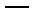
\includegraphics[scale=1]{\figpath/Model1_C2.pdf}\\%& 30 g/mol\\
			Butane & \ce{C4H10} & 
\includegraphics[scale=1]{\figpath/Model1_C4.pdf}\\%& 58 g/mol\\
			Hexane & \ce{C6H14} & 
\includegraphics[scale=1]{\figpath/Model1_C6.pdf}\\%& 86 g/mol\\
			Octane & \ce{C8H18} & 
\includegraphics[scale=1]{\figpath/Model1_C8.pdf}\\%& 114 g/mol\\
			Decane & \ce{C10H22} & 
\includegraphics[scale=1]{\figpath/Model1_C10.pdf}\\%& 142 g/mol
		\end{tabular}
	\end{center}


\end{model}


\begin{ctqs}

	\question Between each line of the table and the next...
		\begin{enumerate}
			\item ... how many carbon atoms are added to the molecule?
			
				\begin{solution}[0.25in]
				2
				\end{solution}
				
			\item ... how many hydrogen atoms are added to the molecule?
			
				\begin{solution}[0.25in]
				4
				\end{solution}
				
		\end{enumerate}
		
	\question Explain, in 1-2 complete sentences, why we might say that this series of molecules consists of ``repeating'' \ce{C2H4} units.
			
				\begin{solution}[1.5in]
					If we ignore the methyl groups on the ends of the chains, we could divide each of the molecules up into a string of \ce{C2H2} units, with one new unit added as we go from one row of the table to the next.  Thus we can think of this series of molecules as consisting of \ce{C2H2} units repeating over and over until we make up the total number of units needed for the chain.
				\end{solution}
				
		
	\question Predict the chemical formula of the next logical entry in the table, and draw its structure.
			
				\begin{solution}[1in]
					The next entry would be \ce{C12H26}:
					
	\instructordisplay{\centerline{
\includegraphics[width=0.3\textwidth]{\figpath/Model1_C12_answer.pdf}}}
				\end{solution}
		
	\question Consider a linear alkane with 100 carbon atoms. \label{\labelbase:ctq:100Calkane}
		\begin{enumerate}
			%\item What would the molecular weight of this molecule be?
			
			\item What would the chemical formula of this molecule be?
			
				\begin{solution}[1in]
					For an alkane with $n$ carbons, the number of hydrogens is $6+2(n-2) = 2n+2$.  Thus a molecule with 100 carbons would have formula\ce{C100H202}.
				\end{solution}
			
			\item Do you \emph{want} to try to draw the full structure of this molecule?  Why or why not?
			
				\begin{solution}[1.25in]
					No!  It would be super long, and really difficult to fit on the page.
				\end{solution}
		\end{enumerate}
\end{ctqs}

\begin{infobox}
	For convenience, large molecules with repeating structures are often abbreviated using the following notation:
	
	\centerline{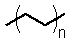
\includegraphics[scale=2]{\figpath/Model1_nrepeats.pdf}}
	
	Here, the repeat unit is enclosed in parentheses.  The repeat units are attached end-to-end, and the subscript $n$ indicates how many times this unit is repeated.  The portions outside of the parentheses are not part of the repeat unit, and indicate the chemical structure of the end-groups that ``cap'' the end of the molecule.
\end{infobox}

\begin{ctqs}
	\question Draw the full structure of the molecule shown in the following abbreviated structure: \label{\labelbase:ctq:abbrevbutane}
	
		\vspace{6pt}
		\centerline{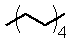
\includegraphics[scale=2]{\figpath/Model1_C10_abbreviated.pdf}}
		
		\begin{solution}[1.25in]
			\instructordisplay{
				\centerline{
\includegraphics[width=0.3\textwidth]{\figpath/Model1_C10_answer.pdf}}
			}
		\end{solution}
	
	\question Propose an analogous abbreviated structure for the 100-carbon linear alkane described in CTQ \ref{\labelbase:ctq:100Calkane}: \label{\labelbase:ctq:abbrev100}
		
		\begin{solution}[0.75in]
			\instructordisplay{
				\centerline{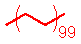
\includegraphics[width=0.1\textwidth]{\figpath/Model1_100C_abbreviated.pdf}}
			}
			Note: common student errors in this question include (1) missing the two carbons contained in the end groups and writing 50 in the subscript, or (2) forgetting that each repeat unit contains two carbon atoms and write 99 or 100 in the subscript.
		\end{solution}
	
	\question What is the chemical formula \emph{of the repeat unit} for the structures in CTQs \ref{\labelbase:ctq:abbrevbutane} and \ref{\labelbase:ctq:abbrev100}?
		
		\begin{solution}[0.75in]
			\ce{C2H4}
		\end{solution}
	
	\question What small molecule has the same chemical formula as this repeat unit?
		
		\begin{solution}[0.75in]
			Ethylene
			
			Note: many students will likely give the IUPAC name, ethene.  If they then get stuck on question 9, it can help to remind them that ``ethylene'' is the common name for this molecule.
		\end{solution}
	
\end{ctqs}

\begin{infobox}
	When the number of repeat units is large, we often describe molecules with repeating structures as \emph{polymers}.  The word polymer comes from Greek: \emph{poly} means ``many'', while \emph{meros} means ``parts''.  Thus, a \emph{polymer} is a molecule composed of \emph{many} (often identical) \emph{parts}.
\end{infobox}

\begin{ctqs}
	\question Why might we describe molecules of the form
	
		\centerline{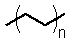
\includegraphics[scale=2]{\figpath/Model1_nrepeats.pdf}}
			
		as \emph{polyethylenes}?  Explain your answer in 1-2 complete sentences.
		
		\begin{solution}[2in]
			We refer to molecules of this form as polyethyelenes because they are made up of many ethylene repeat units.
		\end{solution}
\end{ctqs}

\clearpage
\begin{model}[Melting Points of Linear Hydrocarbons]
	\label{\labelbase:mdl:hydrocarbonmelting}

	The following plot shows the melting points of linear hydrocarbons with varying numbers of carbon atoms:
	
	\vspace{6pt}
	
	\centerline{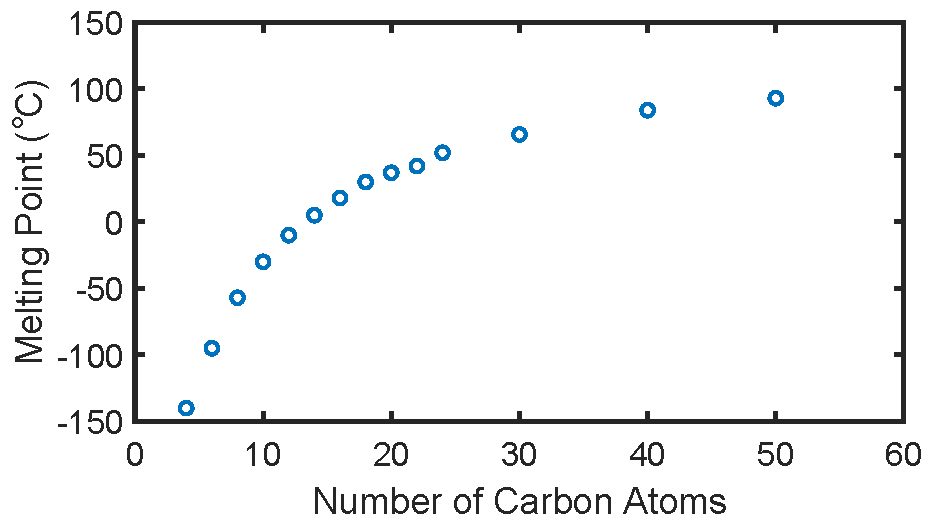
\includegraphics[width=0.7\textwidth]{\figpath/meltingpoints_cleaned.pdf}}
	
	\vspace{6pt}

\end{model}

\begin{ctqs}
	
	\question Consider a sample of ethane molecules.  What type(s) of interactions (e.g. covalent, ionic, hydrogen bonding, van der Waals, etc.) do you expect to govern interactions between these molecules?%, and why?  %Briefly explain your team's reasoning.
	
		\begin{solution}[0.5in]
			Ethane molecules are neither charged nor polar, so they most likely interact through van der Waals interactions.
			
			Note: some students may answer ``covalent''.  Remind these students that the question is asking about interactions \emph{between} chains, not the types of bonds \emph{within} chains.
		\end{solution}
	
	\question As the number of carbon atoms in the molecule increases, do you expect the strength of these intermolecular interactions increase, decrease, or stay the same? \label{\labelbase:ctq:interactionstrength}
	
		\begin{solution}[0.5in]
			Generally, van der Waals interactions increase in strength as molecules become larger and more polarizable, so the interactions between chains should become stronger as the number of carbon atoms in the chain increases.
		\end{solution}
	
	\question Using your answer to CTQ \ref{\labelbase:ctq:interactionstrength}, propose a possible origin for the trend observed in Model \ref{\labelbase:mdl:hydrocarbonmelting} in 1-2 complete sentences.
	
		\begin{solution}[2in]
			As the chains become longer, the interactions between molecules becomes stronger and it takes more energy to melt the material.  Thus, the melting temperature goes up.
		\end{solution}
	
	\question Based on the data presented in Model \ref{\labelbase:mdl:hydrocarbonmelting}, what do you expect to happen to the melting temperature as the number of carbon atoms gets very large (1000 or 10000 or more)?  Briefly explain your team's reasoning.
	
		\begin{solution}[2in]
		
			The data look like they are beginning to level off as the number of carbon atoms increases.  Assuming this trend continues, the melting temperature for very large hydrocarbons is likely to limit somewhere between 100 and 150~${}^\circ$C. 
		\end{solution}
	
	\question The melting temperature of polyethylene is typically quoted as approximately 120~${}^\circ$C.  In your group's judgment, how many carbon atoms are necessary before the melting behavior begins to ``look'' more like the polymer than like a small molecule?  Explain your choice in 2-3 complete sentences. \label{\labelbase:ctq:npolymer}
	
		\begin{solution}[2in]
		
			Student answers will likely vary.  Some may say that it requires 100-500 carbon atoms, because that is where the curve will probably begin to approach 120~${}^\circ$C.  Others may say that it only taks 15-20 carbon atoms, because that is where the slope of the curve really starts to decrease.
			
			In discussion, it is worth emphasizing that the properties of polymers usually change continuously with chain length, and there is no distinct ``cutoff'' that determines when we can start calling something a polymer.  In \emph{practice}, molecules with fewer than 10 repeat units rarely behave like polymers, and are instead referred to as oligomers, while molecules with more than 100 repeat units are usually solidly ``polymer-like''; in between these limits, whether you will see polymer-like or molecule-like behavior depends a lot on which property you are measuring.
			
			(One aspect of this problem is addressed in Exercise 1 of Activity 2, which asks students to consider when end groups do and do not matter on polymer chains.)
		\end{solution}
	
	%\question How many repeat units does this number of carbons correspond to?
	
	%	\begin{solution}[0.5in]
	%	\end{solution}
			
\end{ctqs}

		

\begin{exercises}

	\exercise How many repeat units does the number of carbon atoms you identified in CTQ \ref{\labelbase:ctq:npolymer} correspond to?
	
		\begin{solution}
		
			Student answers will vary, but for $n$ carbon atoms, the corresponding number of repeat units is $(n-2)/2$.
			
		\end{solution}

	\exercise In this class, we will primarily use the word ``polymer'' to describe large molecules with repeating structures.  Another word commonly used in this field, however, is ``macromolecule''.  Why is this also a reasonable term for describing this class of molecules, and does it capture any important features that are missed by the word ``polymer''?
	
		\begin{solution}
			``Macromolecule'' literally means ``large molecule''.  This term is reasonable for describing polymers because they are, in essence, very large molecules, and it emphasizes that the size is the primary feature that distinguishes them from most familiar small molecules.
			
			In practice, we generally use the terms ``macromolecule'' and ``polymer'' interchangeably.  However, it is worth noting that macromolecule is, in some ways, less specific than ``polymer''; a macromolecule can refer to any large molecule, even if it is not made up of repeating parts.  On the other hand, the word ``molecule'' typically refers to collections of atoms that are covalently bonded together, whereas polymer (``many parts'') could feasibly just refer to a collection of loosely associated molecular units, or units that are held together by hydrogen bonds, metal coordination bonds, or other types of non-covalent bonds.  Thus the two terms, while getting at many of the same ideas, are not strictly identical.
		\end{solution}
	
\end{exercises}


%\begin{problems}

%	\problem First exercise
%	\problem Second exercise
	
%\end{problems}


	
\end{activity}